\documentclass[journal,12pt,twocolumn]{IEEEtran}
\newcommand\hmmax{0}
\newcommand\bmmax{0}
\usepackage{dsfont}
\usepackage{setspace}
\usepackage{gensymb}
\singlespacing
\usepackage[cmex10]{amsmath}
\usepackage{relsize}
\usepackage{amsthm}
\usepackage{newtxtext}
\usepackage{mathrsfs}
\usepackage{txfonts}
\usepackage{stfloats}
\usepackage{bm}
\usepackage{cite}
\usepackage{cases}
\usepackage{subfig}
\usepackage{longtable}
\usepackage{multirow}
\usepackage[inline]{enumitem}   
\makeatletter
% This command ignores the optional argument for itemize and enumerate lists
\newcommand{\inlineitem}[1][]{%
\ifnum\enit@type=\tw@
    {\descriptionlabel{#1}}
  \hspace{\labelsep}%
\else
  \ifnum\enit@type=\z@
       \refstepcounter{\@listctr}\fi
    \quad\@itemlabel\hspace{\labelsep}%
\fi}
\makeatother
\usepackage{mathtools}
\usepackage{steinmetz}
\usepackage{tikz}
\usepackage{circuitikz}
\usepackage{verbatim}
\usepackage{tfrupee}
\usepackage[breaklinks=true]{hyperref}
\usepackage{graphicx}
\usepackage{tkz-euclide}
\usepackage{makecell}
\usetikzlibrary{calc,math}
\usepackage{listings}
    \usepackage{color}                                            %%
    \usepackage{array}                                            %%
    \usepackage{longtable}                                        %%
    \usepackage{calc}                                             %%
    \usepackage{multirow}                                         %%
    \usepackage{hhline}                                           %%
    \usepackage{ifthen}                                           %%
    \usepackage{lscape}     
\usepackage{multicol}
\usepackage{chngcntr}
\DeclareMathOperator*{\Res}{Res}

\renewcommand\thesection{\arabic{section}}
\renewcommand\thesubsection{\thesection.\arabic{subsection}}
\renewcommand\thesubsubsection{\thesubsection.\arabic{subsubsection}}

\renewcommand\thesectiondis{\arabic{section}}
\renewcommand\thesubsectiondis{\thesectiondis.\arabic{subsection}}
\renewcommand\thesubsubsectiondis{\thesubsectiondis.\arabic{subsubsection}}
\newcolumntype{C}{>$c<$}

\hyphenation{op-tical net-works semi-conduc-tor}
\def\inputGnumericTable{}                                 %%

\lstset{
%language=C,
frame=single, 
breaklines=true,
columns=fullflexible
}
\begin{document}

\newcommand{\BEQA}{\begin{eqnarray}}
\newcommand{\EEQA}{\end{eqnarray}}
\newcommand{\define}{\stackrel{\triangle}{=}}
\bibliographystyle{IEEEtran}
\raggedbottom
\setlength{\parindent}{0pt}
\providecommand{\mbf}{\mathbf}
\providecommand{\pr}[1]{\ensuremath{\Pr\left(#1\right)}}
\providecommand{\qfunc}[1]{\ensuremath{Q\left(#1\right)}}
\providecommand{\sbrak}[1]{\ensuremath{{}\left[#1\right]}}
\providecommand{\lsbrak}[1]{\ensuremath{{}\left[#1\right.}}
\providecommand{\rsbrak}[1]{\ensuremath{{}\left.#1\right]}}
\providecommand{\brak}[1]{\ensuremath{\left(#1\right)}}
\providecommand{\lbrak}[1]{\ensuremath{\left(#1\right.}}
\providecommand{\rbrak}[1]{\ensuremath{\left.#1\right)}}
\providecommand{\cbrak}[1]{\ensuremath{\left\{#1\right\}}}
\providecommand{\lcbrak}[1]{\ensuremath{\left\{#1\right.}}
\providecommand{\rcbrak}[1]{\ensuremath{\left.#1\right\}}}
\theoremstyle{remark}
\newtheorem{rem}{Remark}
\newcommand{\sgn}{\mathop{\mathrm{sgn}}}
\providecommand{\abs}[1]{\vert#1\vert}
\providecommand{\res}[1]{\Res\displaylimits_{#1}} 
\providecommand{\norm}[1]{\lVert#1\rVert}
%\providecommand{\norm}[1]{\lVert#1\rVert}
\providecommand{\mtx}[1]{\mathbf{#1}}
\providecommand{\mean}[1]{E[ #1 ]}
\providecommand{\fourier}{\overset{\mathcal{F}}{ \rightleftharpoons}}
%\providecommand{\hilbert}{\overset{\mathcal{H}}{ \rightleftharpoons}}
\providecommand{\system}{\overset{\mathcal{H}}{ \longleftrightarrow}}
  %\newcommand{\solution}[2]{\textbf{Solution:}{#1}}
\newcommand{\solution}{\noindent \textbf{Solution: }}
\newcommand{\cosec}{\,\text{cosec}\,}
\providecommand{\dec}[2]{\ensuremath{\overset{#1}{\underset{#2}{\gtrless}}}}
\newcommand{\myvec}[1]{\ensuremath{\begin{pmatrix}#1\end{pmatrix}}}
\newcommand{\mydet}[1]{\ensuremath{\begin{vmatrix}#1\end{vmatrix}}}
\numberwithin{equation}{subsection}
\makeatletter
\@addtoreset{figure}{problem}
\makeatother
\let\StandardTheFigure\thefigure
\let\vec\mathbf
\renewcommand{\thefigure}{\theproblem}
\def\putbox#1#2#3{\makebox[0in][l]{\makebox[#1][l]{}\raisebox{\baselineskip}[0in][0in]{\raisebox{#2}[0in][0in]{#3}}}}
     \def\rightbox#1{\makebox[0in][r]{#1}}
     \def\centbox#1{\makebox[0in]{#1}}
     \def\topbox#1{\raisebox{-\baselineskip}[0in][0in]{#1}}
     \def\midbox#1{\raisebox{-0.5\baselineskip}[0in][0in]{#1}}
\vspace{3cm}
\title{Assignment 7}
\author{Gorantla Pranav Sai- CS20BTECH11018}
\maketitle
\newpage
\bigskip
\renewcommand{\thefigure}{\theenumi}
\renewcommand{\thetable}{\theenumi}

\section{Problem}
\textbf{gov/stats/2015/statistics-I(1), Q.3(C)}\\
  Three points are chosen on the line of unit length.Find the probability that each the 3 line segments have length greater than $\dfrac{1}{4}$.
\section{Solution}
Let $X,Y \in \{0,1\}$ be the random variables which represent the position of two points on the line of unit length.\\
Conditions which should be satisfied to have three line segments with length greater than 
\begin{table}[h]
\centering
\bgroup
\def\arraystretch{2}
\begin{tabular}{|c|c|}
\hline
\textbf{Event} & \textbf{Condition}                     \\\hline
A              & $\dfrac{1}{4}<X<\dfrac{3}{4}$ \\[1ex] \hline
B              & $\dfrac{1}{4}<Y<\dfrac{3}{4}$ \\[1ex] \hline
C              & $\dfrac{1}{4}<|X-Y|$ \\[1ex] \hline
\end{tabular}
\egroup
\caption{Events and their conditions}
\label{tab:Events}
\end{table}
$\frac{1}{4}$ are given in the below table.\\
Then the required event which solves the problem is $ABC$.\\
As $A$ and $B$ are independent events.
\begin{align}
    \pr{ABC}&=\pr{A}\pr{B}\pr{C|AB}
\end{align}
As X and Y are uniformly distributed between 0 and 1.
\begin{align}
    \pr{A}&=\pr{\dfrac{1}{4}<X<\dfrac{3}{4}}=\dfrac{1}{2}\\
    \pr{B}&=\pr{\dfrac{1}{4}<Y<\dfrac{3}{4}}=\dfrac{1}{2}
\end{align}
When event AB is known to occur,X and Y are uniformly distributed between $\dfrac{1}{4}$ and $\dfrac{3}{4}$\\\\ 
Conditional probability density functions of X and Y with condition AB are
\begin{align}
    f_{X|AB}(x) = 
    \begin{cases}
    2 & x\in \brak{\frac{1}{4},\frac{3}{4}}\\
    0 & \text{otherwise}
    \end{cases}
\end{align}
\begin{align}
    f_{Y|AB}(y) = 
    \begin{cases}
    2 & y\in \brak{\frac{1}{4},\frac{3}{4}}\\
    0 & \text{otherwise}
    \end{cases}
\end{align}
Let $Z=X-Y$.Then pdf of Z with condition AB can be given as
\begin{align}
    f_{Z|AB}(z)&=\int_{-\infty}^{\infty}f_{X|AB}(y+z)f_{Y|AB}(y)~dy\\
    f_{Z|AB}(z)&=\int_{\frac{1}{4}}^{\frac{3}{4}}f_{X|AB}(y+z)f_{Y|AB}(y)~dy
\end{align}
if $z \in \sbrak{0,\dfrac{1}{2}}$,
\begin{align}
    f_{Z|AB}(z)&=\int_{\frac{1}{4}}^{\frac{3}{4}-z}f_{X|AB}(y+z)f_{Y|AB}(y)~dy\\
       f_{Z|AB}(z)&=4\brak{\frac{1}{2}-z}\\
       f_{Z|AB}(z)&=2-4z
\end{align}
if$~~z \in \sbrak{-\dfrac{1}{2},0}$,
\begin{align}
    f_{Z|AB}(z)&=\int_{\frac{1}{4}-z}^{\frac{3}{4}}f_{X|AB}(y+z)f_{Y|AB}(y)~dy\\
       f_{Z|AB}(z)&=4\brak{\frac{1}{2}+z}\\
       f_{Z|AB}(z)&=2+4z 
\end{align}
if $~~z \in \brak{-\infty,-\dfrac{1}{2}}\cup \brak{\dfrac{1}{2},\infty}$,
\begin{align}
    f_{Z|AB}(z)=0
\end{align}
\begin{table}[h]
\centering
\bgroup
\def\arraystretch{2}
\begin{tabular}{|c|c|}
\hline
\textbf{Interval} & ${\boldsymbol f_{X|AB}}$                     \\\hline
$z \in \sbrak{0,\dfrac{1}{2}}$       & $2-4z$ \\[1ex] \hline
$~~z \in \sbrak{-\dfrac{1}{2},0}$          & $2+4z$ \\[1ex] \hline
   $~~z \in \brak{-\infty,-\dfrac{1}{2}}\cup \brak{\dfrac{1}{2},\infty}$        & $0$ \\[1ex] \hline
\end{tabular}
\egroup
\caption{Pdf of Z in different intervals}
\label{tab:pdf_Z}
\end{table}
\begin{figure}[h]
    \centering
    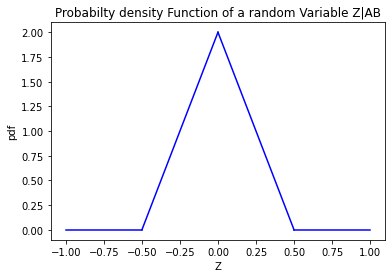
\includegraphics[width=\columnwidth]{figures/pdf_Z.png}
    \caption{pdf Z with AB already occurred}
    \label{fig:pdf_Z}
\end{figure}
\begin{align}
    \pr{C|AB}&=\int_{|z|>\frac{1}{4}}f_{z|AB}~dz\\
             &=\int_{-\frac{1}{2}}^{-\frac{1}{4}}f_{z|AB}~dz+\int^{\frac{1}{2}}_{\frac{1}{4}}f_{z|AB}~dz\\
             &=\dfrac{1}{8}+\dfrac{1}{8}\\
             &=\dfrac{1}{4}
\end{align}
\begin{align}
    \pr{ABC}&=\pr{A}\pr{B}\pr{C|AB}\\
    \pr{ABC}&=\dfrac{1}{2}\times \dfrac{1}{2}\times 
    \dfrac{1}{4}\\
    \pr{ABC}&=\dfrac{1}{16}
\end{align}
$\therefore$ probability that each of the three line segments have length greater than $\dfrac{1}{4}$ is $\dfrac{1}{16}$.
\section{Alternate Method}
 Let $X,Y \in \{0,1\}$ be the random variables which represent the position of two points on the line of unit length.\\
Conditions which should be satisfied to have three line segments with length greater than 
\begin{table}[h]
\centering
\bgroup
\def\arraystretch{2}
\begin{tabular}{|c|c|}
\hline
\textbf{Event} & \textbf{Condition}                     \\\hline
A              & $\dfrac{1}{4}<X<\dfrac{3}{4}$ \\[1ex] \hline
B              & $\dfrac{1}{4}<Y<\dfrac{3}{4}$ \\[1ex] \hline
C              & $\dfrac{1}{4}<X-Y$ \\[1ex] \hline
D           & $\dfrac{1}{4}<Y-X$ \\[1ex] \hline
\end{tabular}
\egroup
\caption{Events and their conditions}
\label{tab:Events}
\end{table}
$\frac{1}{4}$ are given in the below table.\\
Then the required event which solves the problem is $ABC$+$ABD$.
\begin{align}
    \pr{ABC}&=\pr{\frac{1}{4}+Y<X,\frac{1}{4}<X,Y<\frac{3}{4}}\\
    &=\sum~\pr{Y=y|\frac{1}{4}<X,Y<\frac{3}{4}}\times\nonumber\\
    &~~~~~~~~~~\pr{\frac{1}{4}+y<X,\frac{1}{4}<X<\frac{3}{4}}\\
    &=\int_{\frac{1}{4}}^{\frac{3}{4}}dyf_Y(y)\times\nonumber\\ &~~~~~~~\pr{\frac{1}{4}+y<X,\frac{1}{4}<X<\frac{3}{4}}\\
     &=\int_{\frac{1}{4}}^{\frac{3}{4}}dyf_Y(y)\pr{\frac{1}{4}+y<X<\frac{3}{4}}\label{step2}
     \end{align}
     As $X$ is distributed uniformly between 0 and 1.
     \begin{align}
        \pr{\frac{1}{4}+y<X<\frac{3}{4}}=\begin{cases}
        \dfrac{1}{2}-y&y\in \brak{0,\dfrac{1}{2}}\\
        0&\text{otherwise}
        \end{cases}\label{step2help}
     \end{align}
     Using \eqref{step2help},\eqref{step2} can be written as
     \begin{align}
    \pr{ABC}&=\int_{\frac{1}{4}}^{\frac{1}{2}}dyf_Y(y)\brak{\frac{1}{2}-y}
    \end{align}
    As y is distributed uniformly between 0 and 1.
    \begin{align}
   \pr{ABC} &=\int_{\frac{1}{4}}^{\frac{1}{2}}\frac{1}{2}-y~dy\\
    &=\dfrac{1}{32}
\end{align}
Similarly,we can find,
\begin{align}
    \pr{ABD}&=\dfrac{1}{32}
\end{align}
As $C$ and $D$ are mutually exclusive events.
\begin{align}
    \pr{ABC+ABD}&=\pr{ABC}+\pr{ABD}\\
    &=\dfrac{1}{16} 
\end{align}
$\therefore$ probability that each of the three line segments have length greater than $\dfrac{1}{4}$  is  $\dfrac{1}{16}$.
\end{document}    